\documentclass[tikz,border=10pt]{standalone}
\usepackage{libertine}    % Para fuente sans-serif
\renewcommand*\familydefault{\sfdefault} % Fuente principal sans-serif
\usepackage[T1]{fontenc}

\usetikzlibrary{shapes.geometric, arrows.meta, positioning}

\begin{document}
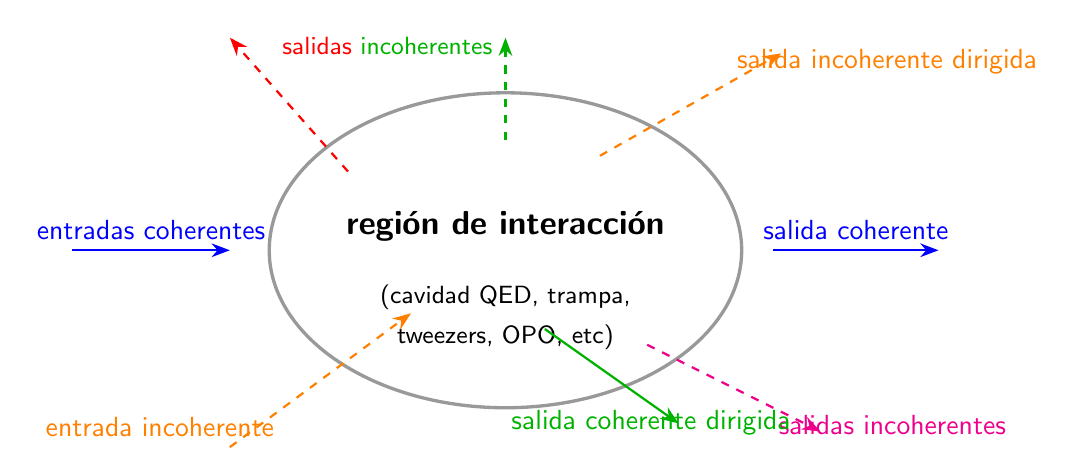
\begin{tikzpicture}[
    >=Stealth,
    font=\sffamily,
    every node/.style={align=center, font=\sffamily},
    linea coherente/.style={draw=blue, thick, ->, solid},
    linea coherente dirigida/.style={draw=green!70!black, thick, ->, solid}, % Verde para coherente dirigida
    linea incoherente entrada/.style={draw=orange, thick, ->, dashed},       % Naranja para entrada
    linea incoherente salida dirigida/.style={draw=orange, thick, ->, dashed}, % Naranja para salida dirigida
    linea incoherente multiple/.style={draw=red, thick, ->, dashed},        % Rojo para múltiple
    linea incoherente multiple abajo/.style={draw=magenta, thick, ->, dashed}, % Magenta para otra múltiple
    linea incoherente arriba verde/.style={draw=green!70!black, thick, ->, dashed} % Verde discontinua para arriba
]

% ---- Elemento central: óvalo (elipse) ----
\draw[draw=gray!50!gray!80, line width=1.2pt, fill=white] 
    (0,0) ellipse [x radius=3cm, y radius=2cm];

% ---- Texto dentro del óvalo ----
\node[font=\sffamily\bfseries, text=black] at (0,0.3) {\large región de interacción};
\node[font=\sffamily\small, text=black] at (0,-0.6) {(cavidad QED, trampa,};
\node[font=\sffamily\small, text=black] at (0,-1.1) {tweezers, OPO, etc)};

% ---- 1. Entrada coherente (izquierda → centro) ----
\draw[linea coherente] (-5.5,0) -- node[above, text=blue, pos=0.5] {entradas coherentes} (-3.5,0);

% ---- 2. Salida coherente (centro → derecha) ----
\draw[linea coherente] (3.4,0) -- node[above, text=blue, pos=0.5] {salida coherente} (5.5,0);

% ---- 3. Entrada incoherente (abajo izquierda → centro) ----
\draw[linea incoherente entrada] (-3.5,-2.5) -- node[below left, text=orange, pos=0.3] {entrada incoherente} (-1.2,-0.8);

% ---- 4. Salida incoherente dirigida (centro → arriba derecha) ----
\draw[linea incoherente salida dirigida] (1.2,1.2) -- node[above right, text=orange, pos=0.7] {salida incoherente dirigida} (3.5,2.5);

% ---- 5. Salidas incoherentes múltiples (parte superior) ----
% Flecha izquierda (rojo)
\draw[linea incoherente multiple] (-2,1) -- (-3.5,2.7);
% Flecha derecha (verde, discontinua)
\draw[linea incoherente arriba verde] (0,1.4) -- (0,2.7);
% Texto para ambas, centrado entre las dos flechas
\node[text=black, font=\sffamily\small] at (-1.5,2.6) {\textcolor{red}{salidas} \textcolor{green!70!black}{incoherentes}};

% ---- 6. Salida incoherente múltiple (abajo derecha, magenta) ----
\draw[linea incoherente multiple abajo] (1.8,-1.2) -- node[below right, text=magenta, pos=0.7] {salidas incoherentes} (4.0,-2.3);

% ---- 7. Salida coherente dirigida (centro → abajo derecha, reposicionada para evitar traslape) ----
\draw[linea coherente dirigida] (0.5,-1.0) -- node[below, text=green!70!black, pos=0.5, xshift=0.5cm, yshift=-0.3cm] {salida coherente dirigida} (2.2,-2.2);

\end{tikzpicture}
\end{document}